\section{Vollständige Induktion}

\morescalingdelimiters

% Induktion Vorstellung
\begin{frame}{Vollständige Induktion}
	Wir haben: Aussage $A_n$ für alle $n \in \N_0$ (z.B. $A_n: \size{\word{a}^n} = n$) \\
	Wir wollen beweisen: $A_n$ ist für alle $n \in \N_0$ wahr \\[0.5em]
	Zeige dazu: \centered{$A_n$ ist für $n = 0$ wahr }
	\centered{\textbf{und}}
	\centered{Wenn $A_n$ für $n$ wahr ist, dann ist $A_n$ auch für $n+1$ wahr}
\end{frame}

\begin{frame}{Vorgehen}
	Behauptung: $\forall n \in \N_0: (n^3 - n) \mod 3 = 0$
	\begin{block}{Induktionsanfang (IA)}
		Beweise die Aussage für die erste Zahl (Basisfall):\\
		$n = 0 \impl (0^3 - 0) \mod 3 = 0 \mod 3 = 0$
	\end{block}
	\begin{block}{Induktionsvoraussetzung (IV)}
		Wir nehmen ein $n$, von dem wir schon gezeigt haben, das die Aussage gilt:\\
		Für ein beliebiges aber festes $n \in \N_0$ gelte: $(n^3 - n) \mod 3 = 0$
	\end{block}
\end{frame}

\begin{frame}{Vorgehen}
	\begin{block}{Induktionsschluss (IS)}
		Zeige die Aussage für $n+1$, verwende dabei die IV:\\
		\begin{align*}
			(n+1)^3 - (n+1) &= n^3 + 3n^2 + 3n + 1 - n - 1\\
			&= (n^3 - n) + (3n^2 + 3n)\\
			&= (n^3-n) + 3 \* (n^2 + n)
		\end{align*}
		$((n^3-n) + 3 \* (n^2 + n)) \mod 3 = \underbrace{(n^3-n) \mod 3}_{\text{nach IV\;} = 0} + \underbrace{3 \* (n^2 + n) \mod 3}_{= 0}$
	\end{block}
	{$\square$ }
\end{frame}

\begin{frame}{Induktionsvoraussetzung}
	\Huge \centering
	Für \textbf{ein} $n \in \N_0$ gelte.\\
	\bigskip
	{ \LARGE
	Nicht: Für alle.\\
	Das wollen wir mit der Induktion erst zeigen!
	}
\end{frame}

\begin{frame}{Vollständige Induktion}
	\begin{itemize}
		\item Der Schraubendreher im Beweis-Werkzeugkasten des Informatikers
		\item Einfaches Prinzip (Verstehen: Reines Auswendiglernen des Schemas führt zu Fehlern!), vielfältige Anwendungsmöglichkeiten
		\item Variationen möglich: Induktionsanfang bei $1, 42, ...$
	\end{itemize}
	
	\FalseQuestionE{Ich benutze für jeden Beweis Induktion.}{Mit einem Schraubendreher bekommt man keinen Nagel in die Wand.}
\end{frame}


\begin{frame}{Zum Aufwärmen: Vogelfarben}
	Wir zeigen nun:\\[2em]
	{\LARGE
	Alle Vögel haben die gleiche Farbe!}\\
	\only<beamer:0>{Achtung: Dieser Beweis enthält selbstverständlich einen Fehler!}
\end{frame}

\begin{frame}{Zum Aufwärmen: Vogelfarben}
	\only<1|handout:1>{
		Dazu verwenden wir \textbf{vollständige Induktion} und zeigen die folgende, äquivalente Aussage: \\
	}
	
	\only<1-3|handout:1-2>{
		\begin{align*}
			 \forall n \in \N_+ : &\text{ In jeder Menge, die genau } n \text{ Vögel enthält,} \\
				&\text{ haben alle Vögel die gleiche Farbe.}
		\end{align*}
	}
	
	\only<2-3|handout:2>{	
		\begin{block}{Induktionsanfang}
			$n = 1$: Wenn eine Menge genau 1 Vogel enthält, dann haben
			offensichtlich alle Vögel die gleiche Farbe.
		\end{block}
	}
	\only<3|handout:2>{
		\begin{block}{Induktionsvoraussetzung}
			Für ein beliebiges aber festes $n$ gelte: In jeder
			Menge, die genau $n$ Vögel enthält, haben alle Vögel die gleiche Farbe.
		\end{block}
	}

	\only<4-5|handout:3-4> {
	\begin{block}{Induktionsschluss}
		\only<4|handout:3>{
			Man zeige die Aussage für $n+1$: Sei also $M$ eine Menge,
			die genau $n+1$ Vögel enthalte. Man stelle sich vor, dass die Vögel
			alle nebeneinander sitzen:
		}
	
		\begin{figure}
			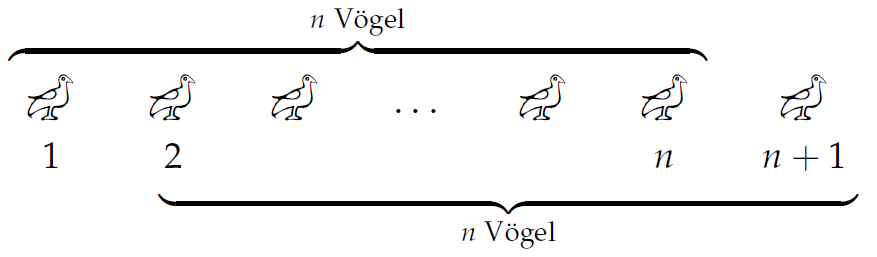
\includegraphics[scale=0.4]{induktion_voegel}
			\centering
		\end{figure}
	
		\only<5|handout:4>{
			Die Vögel $1, 2, ..., n$ bilden eine Menge mit genau $n$ Vögeln. Also haben sie nach Induktionsvoraussetzung alle die gleiche Farbe.\\ 
			Die Vögel $2, 3, ..., n + 1$ bilden auch eine Menge mit genau $n$ Vögeln. Also haben nach Induktionsvoraussetzung auch diese alle die gleiche Farbe.\\
			Folglich haben auch die Vögel $1$ und $n + 1$ die gleiche Farbe, also haben alle Vögel die gleiche Farbe.
		}
	\end{block}
	}
\end{frame}

\begin{frame}{Vogelfarben: Auflösung}
	\begin{figure}
		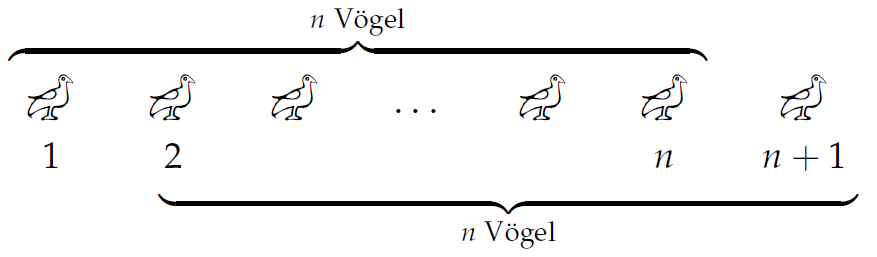
\includegraphics[scale=0.4]{induktion_voegel}
		\centering
	\end{figure}
	Das Bild ist zwar außerordentlich hübsch, suggeriert aber leider etwas, was nicht
	immer stimmt: Für $n = 2$ überlappen sich die Teilmengen „ohne den ersten“ und
	„ohne den letzten“ Vogel nicht. Es ist also nicht erzwungen, dass beide Vögel die
	gleiche Farbe haben.
	(Und das macht „alles weitere“ auch kaputt: Wenn nicht immer 2 Vögel die
	gleiche Farbe haben, dann auch nicht immer 3 Vögel, usw.)
\end{frame}

% Induktion Übung
% -------------------------

\begin{frame}{Und jetzt ihr}
	Behauptung: \[\forall n \in \N_+ : \sum_{k=0}^{n}{\frac{1}{2^k}} = 2 \* (1 - \frac{1}{2^{n+1}})\]
	\begin{block}{Induktionsanfang}
		$n = 1$: $\sum_{k=0}^{1}{\frac{1}{2^k}} = \frac{3}{2} = 2 \* \frac{3}{4}$ \checked
	\end{block}
	\begin{block}{Induktionsvoraussetzung}
		Für ein $n \in \N_0$ gelte: $\sum_{k=0}^{n}{\frac{1}{2^k}} = 2 \* (1 - \frac{1}{2^{n+1}})$
	\end{block}
\end{frame}

\begin{frame}{Und jetzt mit Wörtern}

	\begin{block}{Induktionsschluss}
		Zeige die Aussage für $n+1$:\\
		\begin{align*}
			\sum_{k=0}^{n+1}{\frac{1}{2^k}}
				&= \underbrace{\sum_{k=0}^{n}{\frac{1}{2^k}}}_{\text{IV}} + \frac{1}{2^{n+1}}\\
				&= 2 \* (1 - \frac{1}{2^{n+1}}) + \frac{1}{2^{n+1}}\\
				&= 2 \* (1 - \frac{2}{2^{n+2}} + \frac{1}{2^{n+2}})\\
				&= 2 \* (1 - \frac{1}{2^{(n+1)+1}})
		\end{align*}
	\end{block}
\end{frame}
% -------------------------

% Induktion Wörter Länge
\begin{frame}{Und jetzt mit Wörtern}
	\begin{block}{Behauptung}
		Seien $A, B$ zwei beliebige Alphabete. Definiere die Funktion $f: A^* \to A^*$
		\begin{align*}
			f(\eps) &= \eps \\
			\text{Für } w \in A^*, \mu \in A: f(\mu \· w) &= 
			\begin{cases}
				\mu \· f(w) &\mu \in B \\
				f(w) &\text{sonst}
			\end{cases}\\
		\end{align*}
	
	Dann gilt: $\forall w \in A^*: \size{f(w)} \le \size w$
	\end{block}
\end{frame}

\begin{frame}{Und jetzt mit Wörtern}
	Induktion über die Wortlänge ($n = \size w$):\\[0.5em]
	\begin{block}{Induktionsanfang}
		$n = 0$: Nur das leere Wort hat Länge 0. Also $w = \eps$\\
		$f(\eps) = \eps \impl \size{f(w)} = \size w = 0$
	\end{block}
	\begin{block}{Induktionsvoraussetzung}
		Für ein $n \in \N_0$ gelte: Für alle Wörter der Länge $n$ über $A$ (also $w \in A^n$) ist $\size{f(w)} \le \size w$
	\end{block}
\end{frame}

\begin{frame}{Und jetzt mit Wörtern}

	\begin{block}{Induktionsschluss}
		Zeige die Aussage für $n+1$:\\
		Sei $w \in A^{(n+1)}$ ein Wort der Länge $n+1$.\\
		Dann teilen wir es auf in $w = \mu \· v$ wobei $\mu \in A$ und $v \in A^n$.\\
		Nach IV gilt: $\size{f(v)} \le \size v$\\
		Fall 1: $\mu \in B$: $f(w) = \mu \· f(v)$ \impl $\size{f(w)} = 1 + \size{f(v)} \le 1 + \size v = 1+n = \size w$\\
		Fall 2: $\mu \notin B$: $f(w) = f(v)$ \impl $\size{f(w)} = \size{f(v)} \le \size v = n \le n+1 = \size w$\\
		\smallskip
		Also gilt: $\size{f(w)} \le \size w$
	\end{block}
\end{frame}